% The three test surfaces of Section~\ref{sec:testfunctions}, drawn by hand.
% Input by textbook.tex; a sketch and not a rendered figure, so it is outside
% the figure cache and the render cap, which govern generated output only.
% It carries no factor graph --- the section states no model over
% variables --- so it does not use the shared vocabulary of preamble.tex;
% what is drawn is the shape of each surface.
\begin{figure}[htbp]
\centering
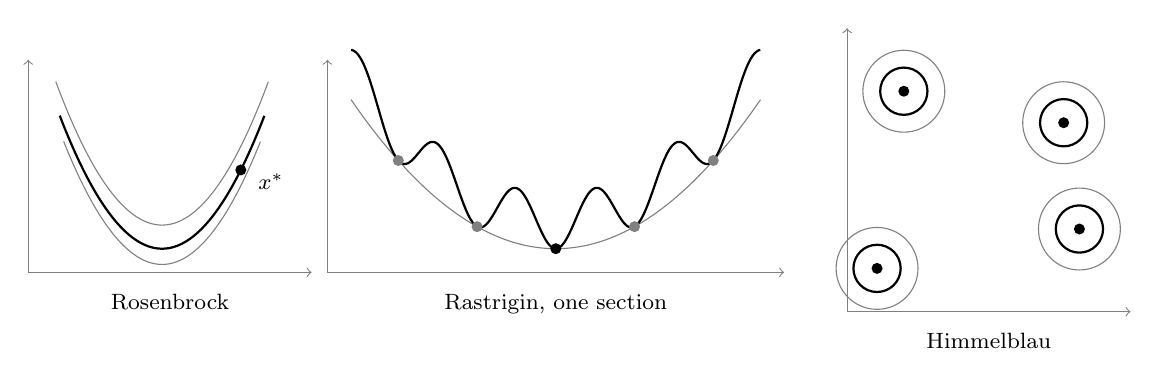
\begin{tikzpicture}[
    scale=1.0,
    curve/.style={draw, thick},
    faint/.style={draw, thin, gray},
    minimum/.style={circle, fill=black, minimum size=0.14cm, inner sep=0pt},
    axis/.style={draw, ->, thin, gray}
]
  % --- Rosenbrock: one curved valley, conditioning and nothing else -------
  \begin{scope}[xshift=0cm]
    \draw[axis] (-1.7, -0.3) -- (1.9, -0.3);
    \draw[axis] (-1.7, -0.3) -- (-1.7, 2.4);
    \draw[faint, domain=-1.35:1.35, samples=80] plot (\x, {\x*\x + 0.30});
    \draw[faint, domain=-1.25:1.25, samples=80] plot (\x, {\x*\x - 0.20});
    \draw[curve, domain=-1.3:1.3, samples=80] plot (\x, {\x*\x});
    \node[minimum] at (1.0, 1.0) {};
    \node[font=\footnotesize, anchor=west] at (1.1, 0.85) {$x^{\ast}$};
    \node[font=\footnotesize, anchor=north] at (0.1, -0.45) {Rosenbrock};
  \end{scope}
  % --- Rastrigin: a bowl under a ripple, one section of it ---------------
  \begin{scope}[xshift=5.0cm]
    \draw[axis] (-2.9, -0.3) -- (2.9, -0.3);
    \draw[axis] (-2.9, -0.3) -- (-2.9, 2.4);
    \draw[faint, domain=-2.6:2.6, samples=80] plot (\x, {0.28*\x*\x});
    \draw[curve, domain=-2.6:2.6, samples=260]
      plot (\x, {0.28*\x*\x - 0.35*cos(360*\x) + 0.35});
    \node[minimum] at (0, 0) {};
    \foreach \x in {-2,-1,1,2} { \node[minimum, fill=gray] at (\x, {0.28*\x*\x}) {}; }
    \node[font=\footnotesize, anchor=north] at (0, -0.45) {Rastrigin, one section};
  \end{scope}
  % --- Himmelblau: four basins of equal depth ----------------------------
  \begin{scope}[xshift=10.4cm, yshift=0.9cm]
    \draw[axis] (-1.7, -1.7) -- (1.9, -1.7);
    \draw[axis] (-1.7, -1.7) -- (-1.7, 1.9);
    \foreach \cx/\cy in {1.05/0.70, -0.98/1.10, -1.32/-1.15, 1.25/-0.65} {
      \draw[faint] (\cx, \cy) circle (0.52);
      \draw[curve] (\cx, \cy) circle (0.30);
      \node[minimum] at (\cx, \cy) {};
    }
    \node[font=\footnotesize, anchor=north] at (0.1, -1.85) {Himmelblau};
  \end{scope}
\end{tikzpicture}
\caption{The three surfaces, schematically. Rosenbrock is a single curved
valley whose difficulty is conditioning alone, and its minimizer is the
marked point of Equation~\ref{eq:rosenbrock}. Rastrigin, drawn as one
one-dimensional section, is a quadratic bowl under a cosine ripple: the black
point is the global minimum of Equation~\ref{eq:rastrigin} and every grey
point a local minimum satisfying the same first-order condition, of which
there are about $10^d$ in $d$ dimensions. Himmelblau has four minima of equal
value, Equation~\ref{eq:himmelblau}, so ``the'' optimum is not a well-formed
question and a method that always returns one basin is reading its start. A
sketch of the shape of each surface, not a rendering of any of them; the
rendered surfaces are Figure~\ref{fig:optimizer-landscapes}.}
\label{fig:testfunctions:sketch}
\end{figure}
